\documentclass[notheorems,mathserif,table,compress]{beamer}  %dvipdfm选项是关键,否则编译统统通不过
%%------------------------常用宏包------------------------
%%注意, beamer 会默认使用下列宏包: amsthm, graphicx, hyperref, color, xcolor, 等等
\usepackage{fontspec,xunicode,xltxtra}  % for XeTeX
\usepackage{verbatim}
\usepackage{mathabx}
%%------------------------ThemeColorFont------------------------
%% Presentation Themes
% \usetheme[<options>]{<name list>}
\usetheme{Madrid}
%% Inner Themes双精度计算
% \useinnertheme[<options>]{<name>}
%% Outer Themes
% \useoutertheme[<options>]{<name>}
\useoutertheme{miniframes} 
%% Color Themes 
% \usecolortheme[<options>]{<name list>}
%% Font Themes
\usefonttheme{serif}
\setbeamertemplate{background canvas}[vertical shading][bottom=white,top=structure.fg!7] %%背景色, 上25%的蓝, 过渡到下白.
\setbeamertemplate{theorems}[numbered]
\setbeamertemplate{navigation symbols}{}   %% 去掉页面下方默认的导航条.
\usepackage{zhfontcfg}
%\setsansfont[Mapping=tex-text]{文泉驿正黑}  %% 需要fontspec宏包
     %如果装了Adobe Acrobat,可在font.conf中配置Adobe字体的路径以使用其中文字体
     %也可直接使用系统中的中文字体如SimSun,SimHei,微软雅黑 等
     %原来beamer用的字体是sans family;注意Mapping的大小写,不能写错
     %设置字体时也可以直接用字体名,以下三种方式等同:
     %\setromanfont[BoldFont={黑体}]{宋体}
     %\setromanfont[BoldFont={SimHei}]{SimSun}
     %\setromanfont[BoldFont={"[simhei.ttf]"}]{"[simsun.ttc]"}
%%------------------------MISC------------------------
\graphicspath{{figures/}}         %% 图片路径. 本文的图片都放在这个文件夹里了.
%%------------------------正文------------------------
\begin{document}
\XeTeXlinebreaklocale "zh"         % 表示用中文的断行
\XeTeXlinebreakskip = 0pt plus 1pt % 多一点调整的空间
%%----------------------------------------------------------
%% This is only inserted into the PDF information catalog. Can be left
%% out.
%%%
%% Delete this, if you do not want the table of contents to pop up at
%% the beginning of each subsection:
\AtBeginSection[]{                              % 在每个Section前都会加入的Frame
  \frame<handout:0>{
    \frametitle{Contents}\small
    \tableofcontents[current,currentsubsection]
  }
}

\AtBeginSubsection[]                            % 在每个子段落之前
{
  \frame<handout:0>                             % handout:0 表示只在手稿中出现
  {
    \frametitle{Contents}\small
    \tableofcontents[current,currentsubsection] % 显示在目录中加亮的当前章节
  }
}

%%----------------------------------------------------------
\title{Saliency Detection}
\subtitle{Weekly Report}
\author[zhu]{\textcolor{olive}{ZhuYafei}}
\institute[OUC]{\small\textcolor{violet}{Ocean University of China}\\
\small\textcolor{violet}{College of Information Science and Engineering}}
\date{August 8, 2014}
%\titlegraphic{\vspace{-6em}\includegraphics[height=7cm]{ouc}\vspace{-6em}}
\frame{ \titlepage }
%%----------------------------------------------------------


%%----------------------------------------------------------
\begin{frame}
  \begin{figure}[!ht]
  \begin{minipage}[t]{0.3\textwidth}
  \centering
  
\includegraphics[width=1in]{cropped_15.png}
  \end{minipage}
  \begin{minipage}[t]{0.3\textwidth}
  \centering
  
\includegraphics[width=1in]{cropped_29.png}
  \end{minipage}
  \begin{minipage}[t]{0.3\textwidth}
  \centering
  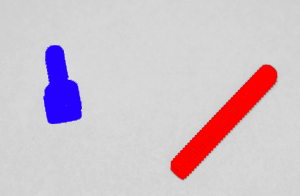
\includegraphics[width=1in]{cropped_31.png}
  \end{minipage}
  \caption{Labeled by three different subjects}
  \end{figure} 
  
  \begin{figure}[h]
  \centering
  \centerline{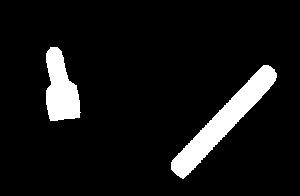
\includegraphics[width=1in]{cropped.png}}
  \caption{GroundTruth}
  \end{figure}
\end{frame}


\begin{frame}
  \begin{figure}[h]
  \centering
  \centerline{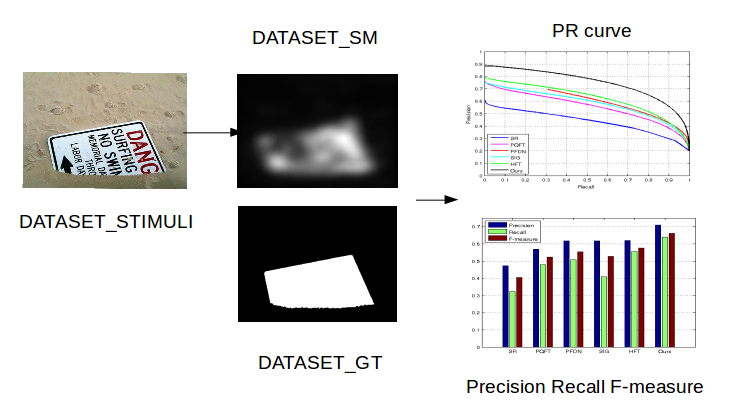
\includegraphics[width=10cm]{img.png}}
  \end{figure}
\end{frame}


\begin{frame}
  \frametitle{Plans}
\begin{enumerate}
  \item Modify the evaluation codes and then push them to github.
  \item Evaluate all the models on all the datasets.
  \item Learn other models and run them.
\end{enumerate}
\end{frame}

\end{document}
